%data
\section{Point Source Tracks Sample} \label{sec:data}
%which dataset to use and why\\
%description of the set: table of various info (livetime, number of events)\\
%mention overlap in time due to testruns\\
%
%This dataset is based on Tessa's sample
%
%ps\_tracks version-p04-00
%
%general changes:
%More precise GRL because subruns that have been missing due to prevoius processing have been accounted for.
%It does not require the TruncatedEnergy fit to be successful leading to around 1\% more events than in prevous samples
%general improvements:
%pass 2 data and new mc file
%unified processing for the datasets from 2011 to 2019

The dataset used in this analysis is a subset of the so-called Point Source Tracks sample, which was first introduced in 2017 and has since undergone several, altogether about 14, revised versions.
Specially optimized for point source searches, this sample of muon neutrinos is the first port of call for analyses of this kind.
The analysis in this work uses 9 years of version p04-00, which is the latest stable version of the datasets since this work began.
This version contains $\SI{1}{\percent}$ more data than its predecessors because the truncated energy fit no longer needs to be successful.
It also contains a more precise good run list, since some subruns were lost in previous versions, which have now been taken into account.
Although this version has 12 years of data, only the years after IC79 are used in this analysis, as the use of earlier datasets is discouraged\footnote{This information stems from the dataset description and several presentations on updates to these sets.}.
The key features of the data used can be seen in table \ref{tab:data}.

\begin{table}
  \centering
  \caption{Number of events and livetimes taken from the good run list of the used datasets in this analysis.}
  \begin{tabular}{lcc}
    \toprule
    Dataset & No. of events & Livetime in days \\
    \toprule
    IC86, 2011 & 119169 & 340.07 \\
    IC86, 2012 & 116715 & 327.70 \\
    IC86, 2013 & 126337 & 355.57 \\
    IC86, 2014 & 129823 & 365.52 \\
    IC86, 2015 & 130434 & 365.27 \\
    IC86, 2016 & 126438 & 357.16 \\
    IC86, 2017 & 145602 & 405.63 \\
    IC86, 2018 & 129230 & 362.54 \\
    IC86, 2019 & 109616 & 304.70 \\
    \hline
    Total & 1133364 & 3184.16 \\
    \toprule
    \label{tab:data}
  \end{tabular}
\end{table}

The temporal intervals of the samples overlap with each other due to testruns of the detector.
There is however no real temporal overlap of the different runs \cite{private_com}.
The advantage of using the years 2011 to 2019 is that the sets have all gone through the same processing pipeline and also all use the same Monte Carlo (mc) file, and thus can be treated the same.

\section{Monte Carlo Pre-Processing}
%removing sources from data and mc\\
%show sindec distribution of mc and filtered mc, maybe sindec-energy 2d hist\\
%mention weighting (Powerlawflux)\\

Since GFU-gold events are treated as sources, keeping these events in the dataset would lead to a bias, due to essentially double counting them as events and sources.
Alert events in general are excluded from the Point Source Tracks Sample starting with IC86.
Some alerts do appear in IC79 and previous runs because these datasets are too old, but are excluded in this analysis since it starts with the year 2011.
Following a conservative approach, GFU-gold events also have to be identified and removed from the simulation files.
Luckily all datasets from the years 2011 to 2019 use the mc file from the year 2016, so this is the only simulation set that needs to be adapted.

To identify the GFU-gold events from the mc set, the original i3 simulation files and the corresponding geometry file (GCD: geometry, calibration, detector configuration) need to be found and processed using the alertfilter from \texttt{realtime}.
The matching simulation files are 21002 and 21220.
%Information about these sets can be found at \cite{sim} and \cite{gcd} for the geometry file.
It is important to mention that the events in the final mc set cannot be identified by their ids since these values were replaced by the job-id of the corresponding analysis pipeline which processed these to the final level.
An exception is the run-id.
The temporal parameter can also not be used, since all event times in the final mc are set to \num{0}.
The event times will be generated later in the analysis to match the analysis framework.
The identification has to be done via other parameters like zenith and azimuth.
Additionally, the true energy was also taken as an identifying parameter to rule out any events coincidentally appearing from the same direction.
A comparison of the $\sin{(\delta)}$ distribution of the real GFU-gold alerts and the GFU-gold simulation events can be seen in figure \ref{fig:gfu_gold_comp}.
In addition, a comparison of the reconstructed energy is given in figure \ref{fig:gfu_gold_comp_energy}.
\begin{figure}
    \centering
    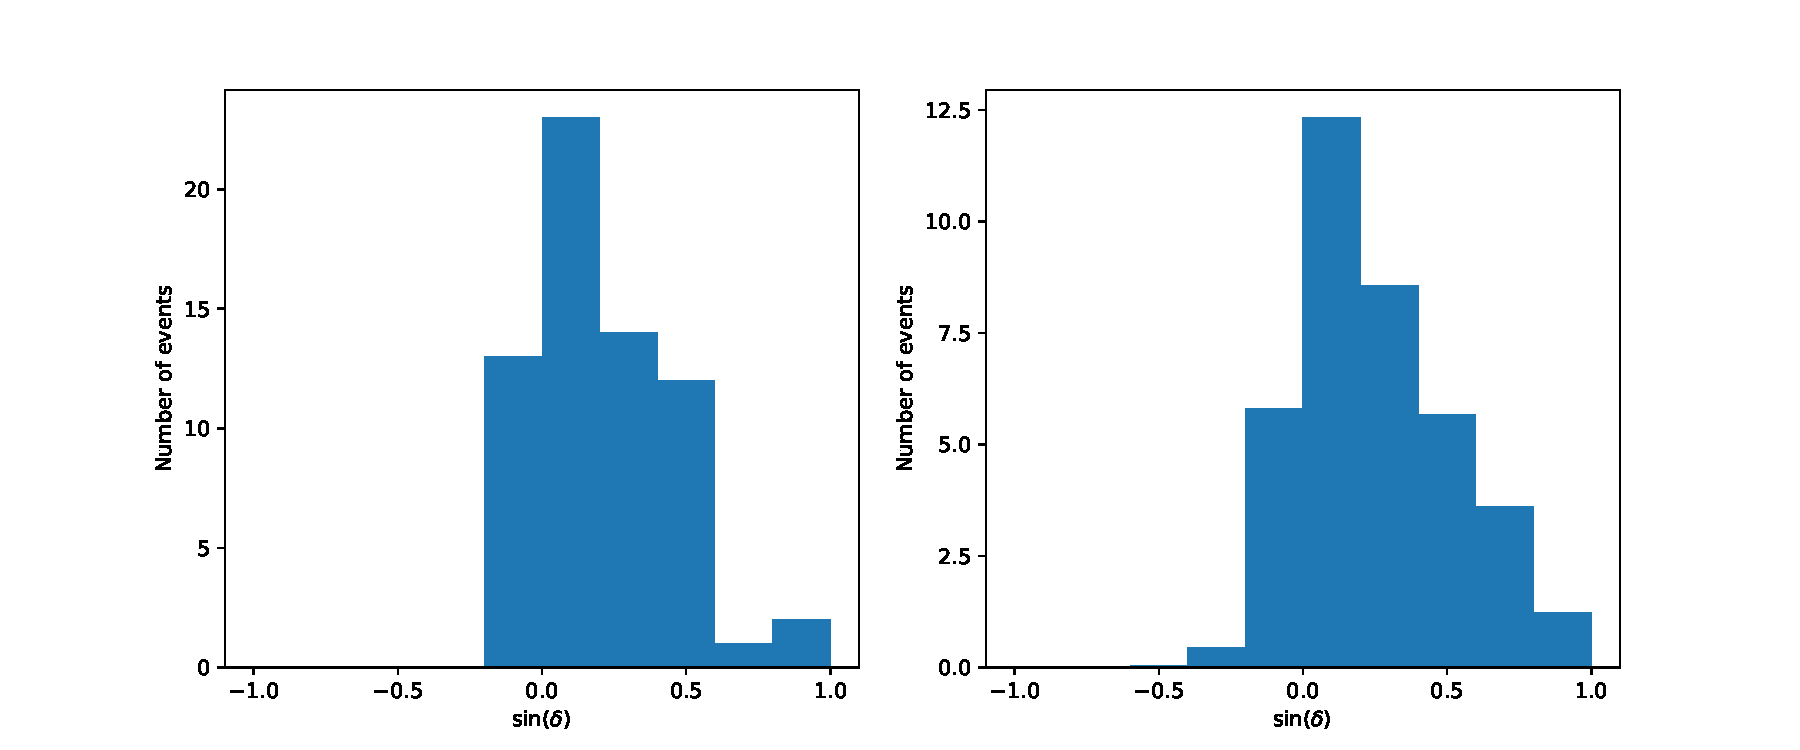
\includegraphics[width=12cm]{Plots/03_data/gfu_gold_comp.pdf}
    \caption{The $\sin{(\delta)}$ of the real GFU-gold alerts over 9 years used in this analysis (left) and the GFU-gold simulation events from the mc 2016 sample (right). The simulation events have been weighted with a livetime of 9 years and flux from \cite{flux}.}
    \label{fig:gfu_gold_comp}
\end{figure}
\begin{figure}
    \centering
    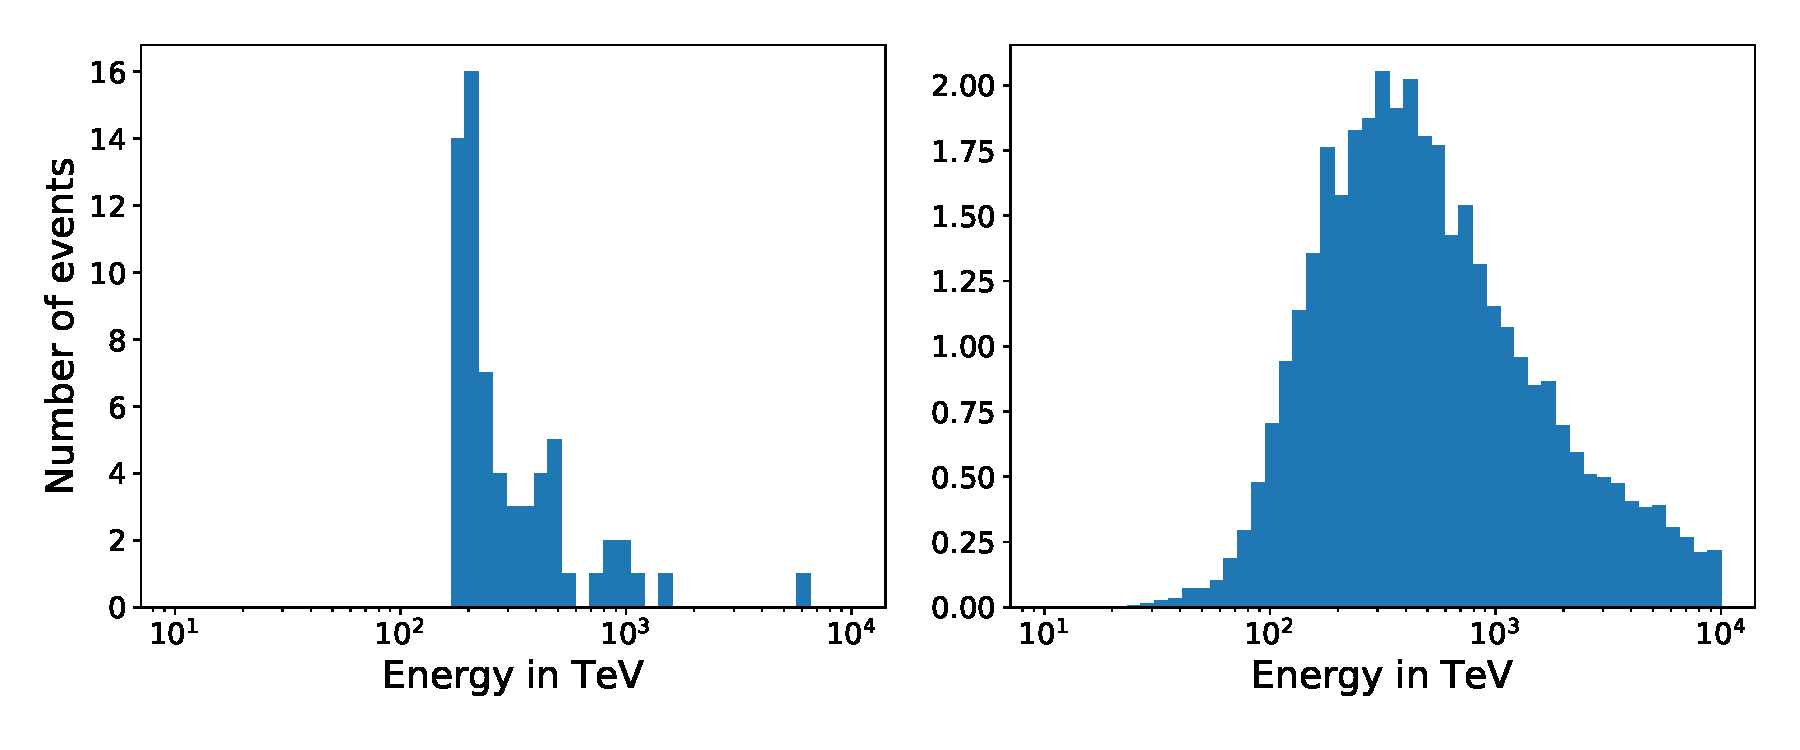
\includegraphics[width=12cm]{Plots/03_data/gfu_gold_energy_comp.pdf}
    \caption{The energy of the real GFU-gold alerts over 9 years used in this analysis (left) and the reconstructed energy of the GFU-gold simulation events from the mc 2016 sample (right). The simulation events have been weighted with a livetime of 9 years and flux from \cite{flux}.}
    \label{fig:gfu_gold_comp_energy}
\end{figure}

Though the mc seems to have about twice as many events the overall form of the $\sin{(\delta)}$ distribution is the same.
However, it is noticeable that the energy distribution of the simulation events is about one order of magnitude too small.
Due to time constraints, the explanation for this shift could not be found.
Presumably, this phenomenon is caused by unequal energy estimators or an incorrect weighting.
In terms of their energy the filtered-out events can also be seen in figure \ref{fig:energy}.
Overall not a lot of events get filtered out, which is to be expected given their nature of being GFU-gold events.
These events are mostly upgoing with high energy.
Since not many events are affected, the energy shift, which can be observed in figure \ref{fig:gfu_gold_comp_energy}, will not have a severe impact on the results.
\begin{figure}
    \centering
    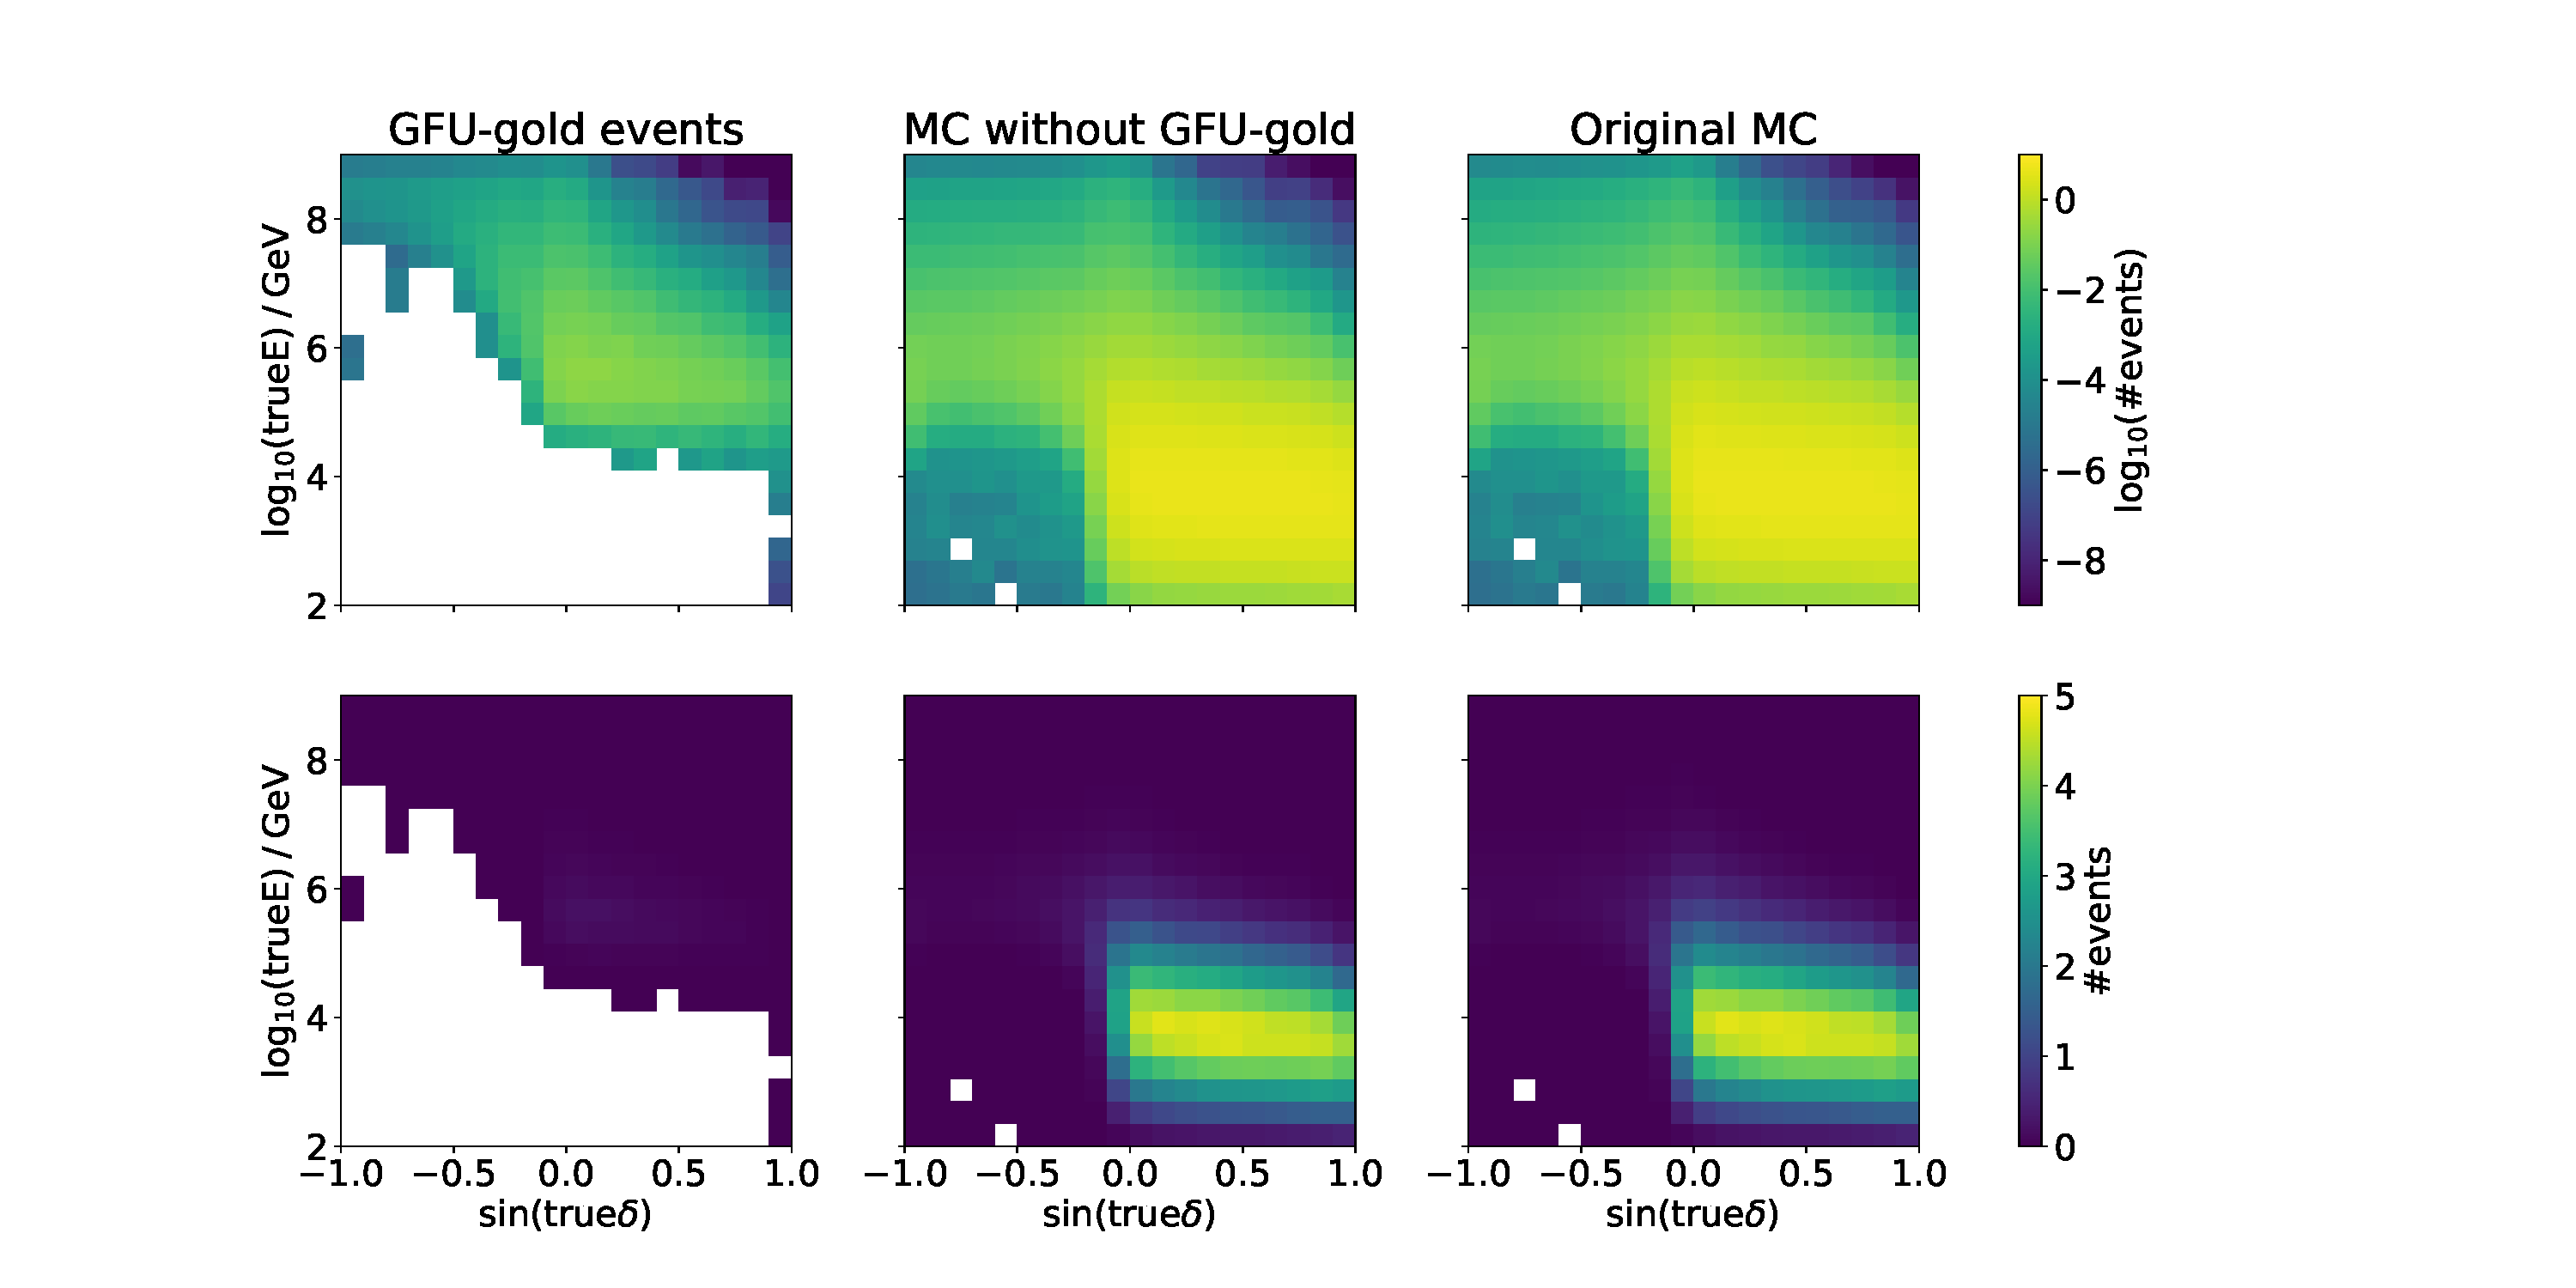
\includegraphics[width=16cm]{Plots/03_data/cleaned_mc_energy_test.pdf}
    \caption{One year weighted histogram in $\log_{10}(\text{trueE})$ and $\sin{(\text{true}\delta)}$ of the GFU-gold events (left column), the mc without the GFU-gold events (middle column) and the original mc with all events (right column) on a logarithmic scale (top row) and on a linear scale (bottom row) for the 2016 mc set. The flux used for the weighting is the same as in figure \ref{fig:gfu_gold_comp}.}
    \label{fig:energy}
\end{figure}
